\documentclass{article}
\usepackage{graphicx}
\begin{document}

\title{JOURNAL FOR LiDAR-VISION}
\author{Ayush Nayak}
\date{\today}

\maketitle

\begin{abstract}
    This is just the daily journal of my musings with this project, and where it will go. hanks!
\end{abstract}

\newpage

\section{June 25th}

This is the day that I started the journal, and started coding in the basic \LaTeX. The basic outline for the project, is to use LiDAR sensors to take in the surroundings, and then feed that into a computer, which determines all the obstacles, and then translates them into sound, which is played back through Dolby Atmos. The entire thing should be able to be compacted into a single pair of glasses, with a small LiDAR detector on top.

\section{June 29th}

The new Air Pods Pro feature is a must, where it has surround sound, as well as gyroscopes to show where everything is.

If I ever get serious about this, Airpods Pro + an iPhone XR and a LiDAR Helmet piece would probably be perfect. Dolby Atmos support is also pretty awesome, maybe WM300 XM3. Surround Sound + Lidar Detection, although I'm not super sure about how useful it would be to have lidar input, and how easy it is to differentiate different objects.

\section{June 30th}
So I am going to split this into two parts.

The first part is the actual LiDAR point detection and image classification, while the second type is the actual translating that LiDAR image into objects and classifying them. The second part is to actually take that plane of classified images, and turn it into audio signals through Dolby Atmos. 

Each day, I will just mark Part 1, and Part 2, and update each one individually. 

\textbf{Part 1:}

First, in order to detect whats going on, 3D and 2D classification will be used, preferably, through the KITTI dataset for 3d and 2d objects, through C++ for super fast execution, as this will have to happen on my terrible i7 5700xt for AI. Maybe use TensorFlow Lite C++ to train an embedded package. 
- I will have to build a camera detection system that can detect basically any object, using open source datasets, and then verify that object with the LiDAR Sensor, which may be more optional, although is more for distance than actual image classification. 

A diagram of the different classification and warning sites can be shown below.
\begin{figure}[htbp]
    \centerline{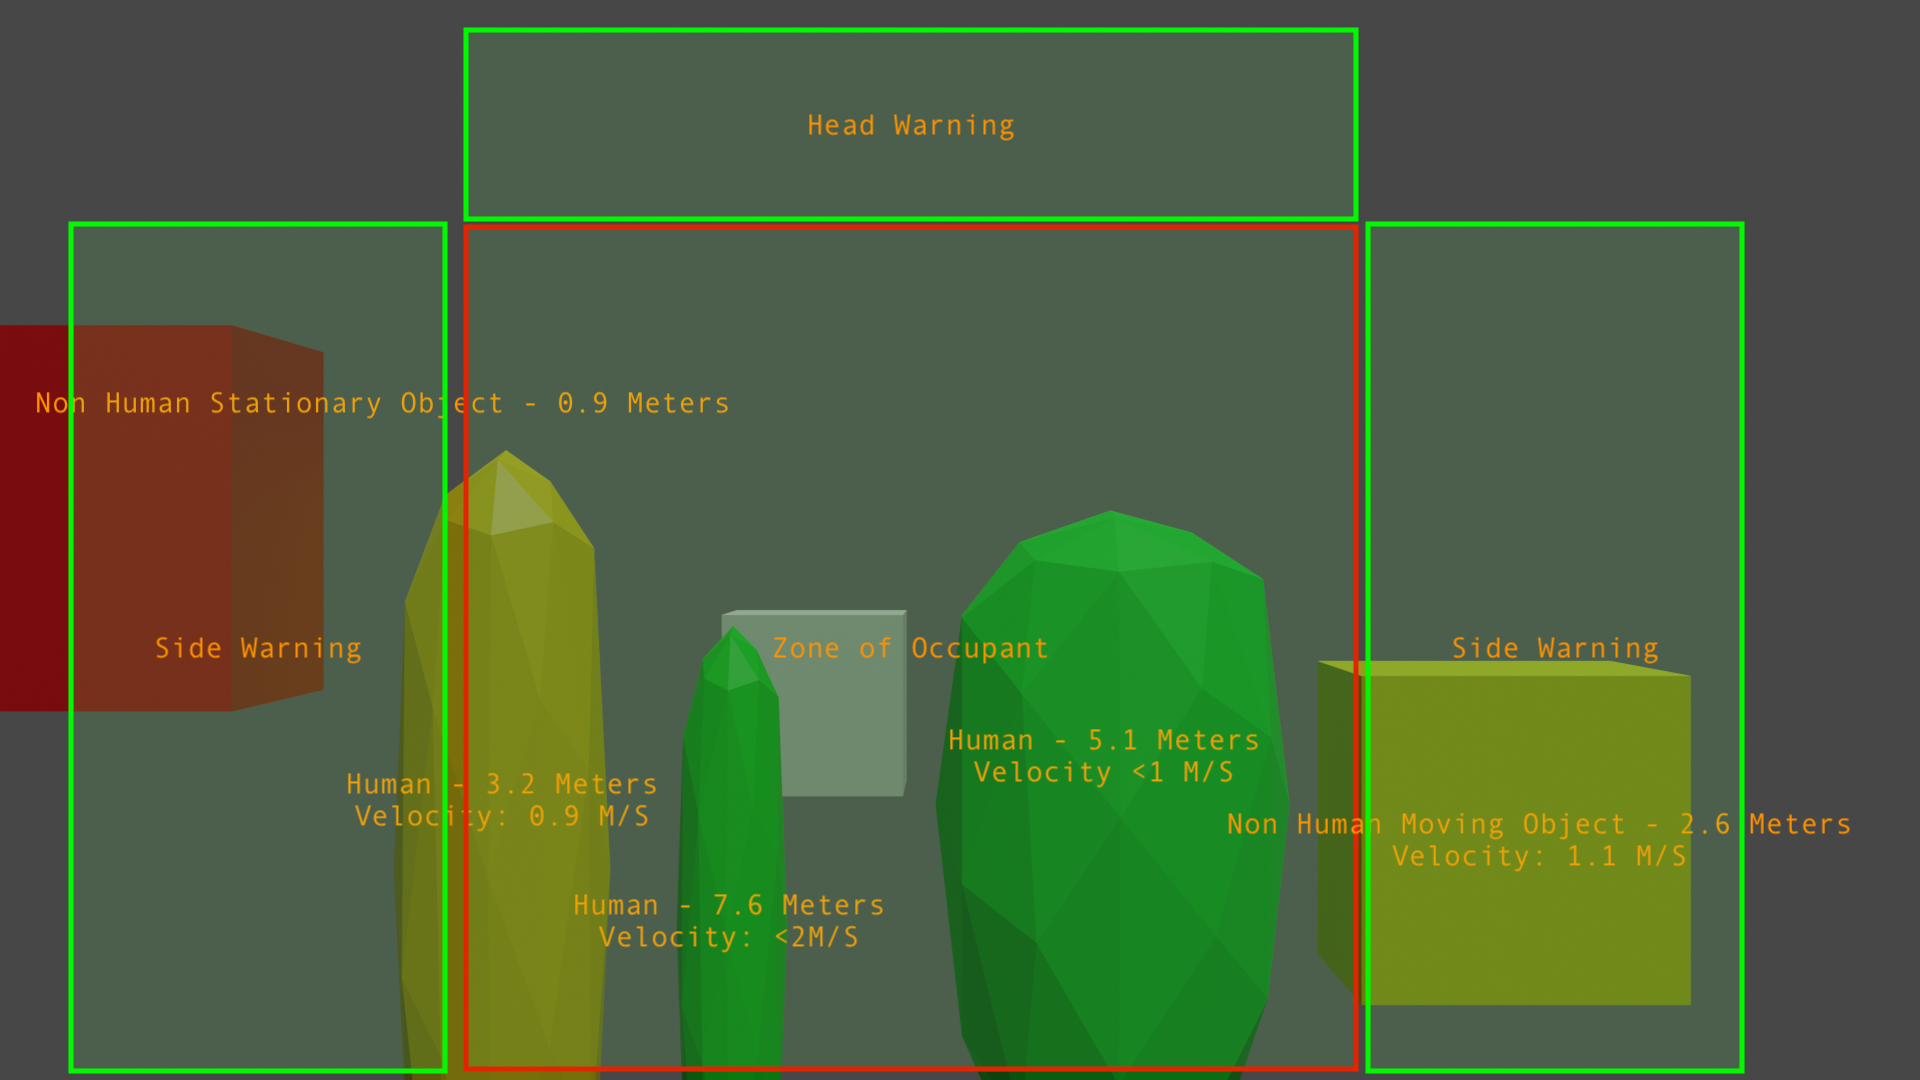
\includegraphics[scale=0.1]{Images/topviewtestsfrontview0.png}}
    \caption{This is a front view of classification space. At a basic level, things are classified as Humans, Cars, Stationary Objects, and Moving Objects. Different stages of warning are given.}
    \label{fig1}
\end{figure}

\begin{figure}[htbp]
    \centerline{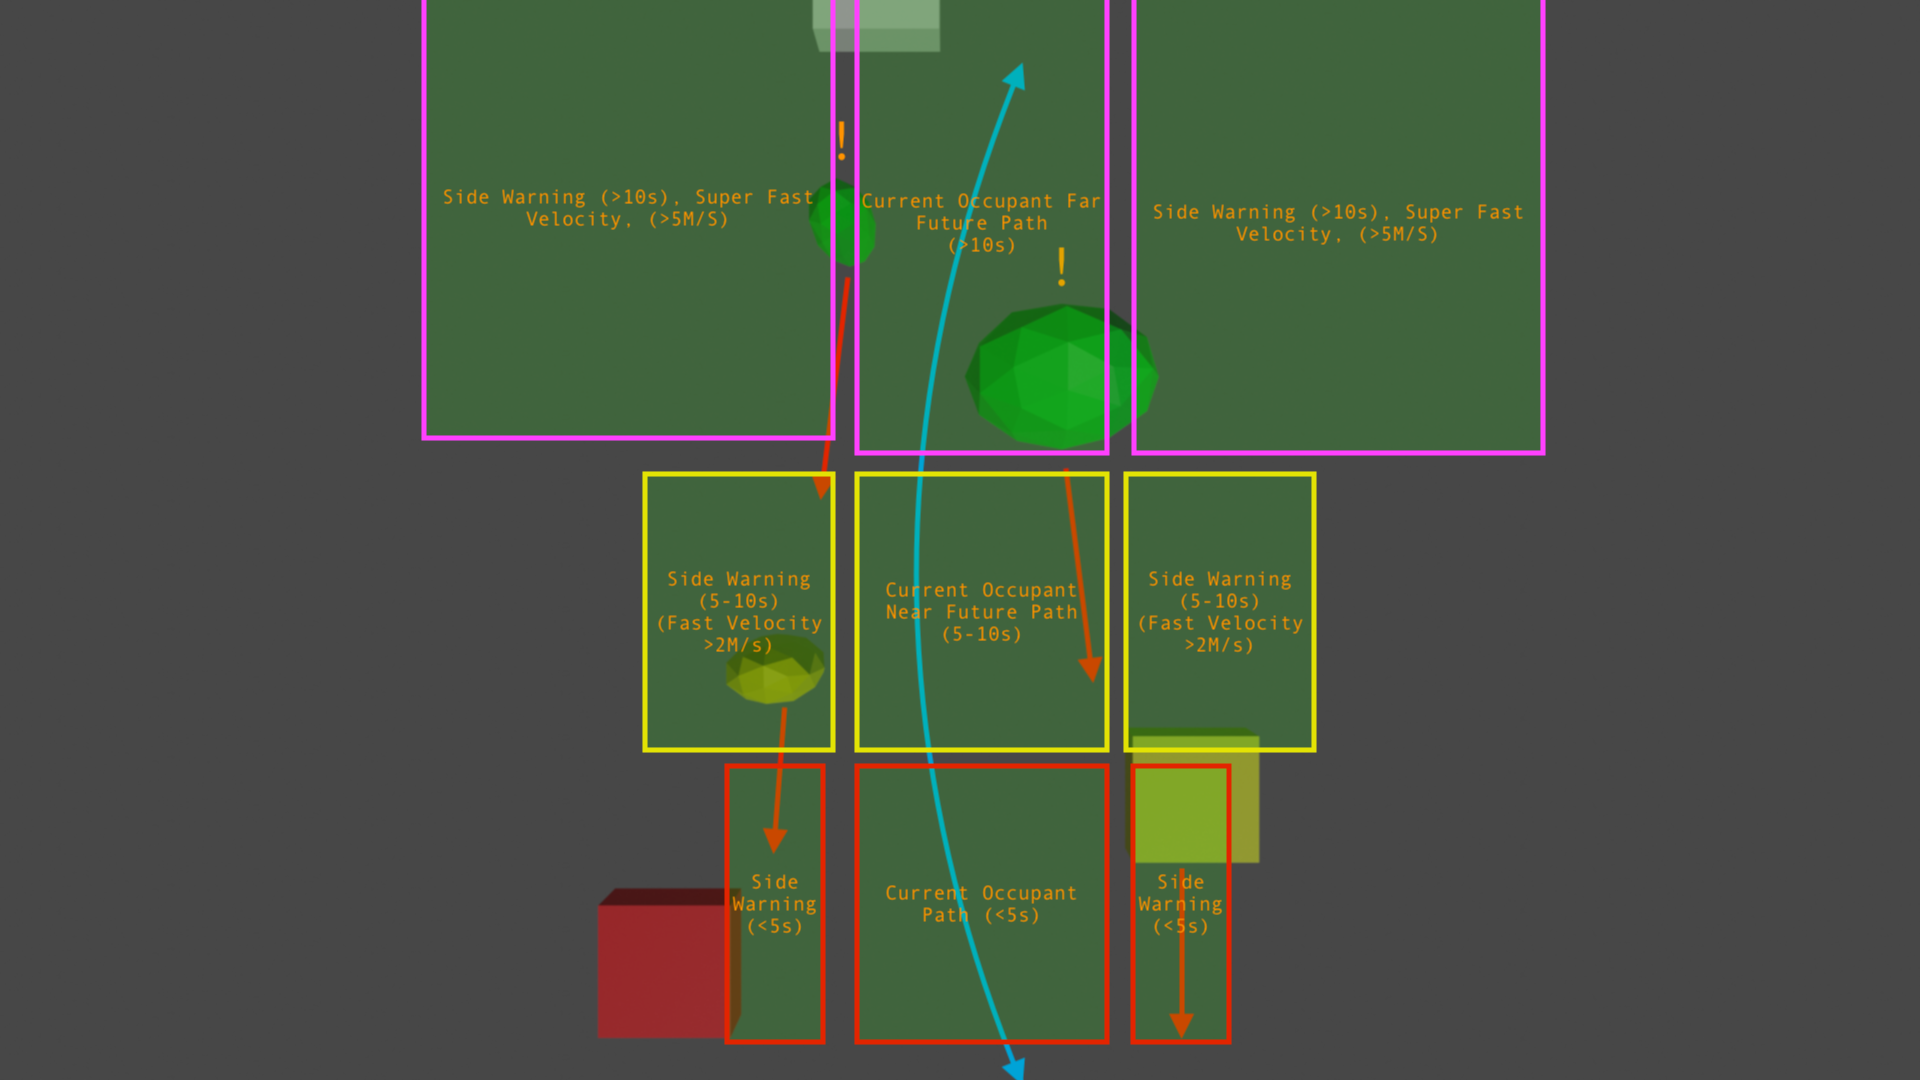
\includegraphics[scale=0.1]{Images/topviewtestset0.png}}
    \caption{This is a top view of classification space. At a basic level, things are classified as Humans, Cars, Stationary Objects, and Moving Objects. Different stages of warning are given, and here one can see why LiDAR is needed, as even for humans, it is very tricky to tell the distance of objects from the top perspective picture without labels}
    \label{fig2}
\end{figure}

For basic classification, a minimum amount of classes are needed, summarized in the table below

\begin{tabular}{ |p{2.5cm}||p{2.8cm}||p{1.8cm}||p{2.45cm}|  }
    \hline
    \multicolumn{4}{|c|}{Different categories for ultrabasic image classification } \\
    \hline
    Moving & Ground Changes & Stationary & Humans\\
    \hline
    \hline
    Cars            & Slope             & Pole      & Stationary\\
    Bikes           & Large Bump        & Booth     & Medium Fast\\
    Wheeled Object  & Small Bump        & Store     & Drunk/Random\\
    Large Pushcart  & Dropped Obstacle  & Hydrant   & Signaling\\
    Scooter         & Fluid             & Zoned Area& \\
    Animal          & Texture Change    & Door      & \\
    Other Moving    & Place to Stop     &           & \\
                    & Other             &           & \\
    \hline
\end{tabular}

    
Classification for these objects will be in two ways, first of all, if they are moving, velocity, and expected path, and how it conflicts with the current movers path, this can be seen in the second image. Secondly, identifying the type of change, whether it is in range, and then accordingly warning the occupant.

\section{July 1st}

\textbf{Part 1:}

Training the AI to recognize the background, through a combination of LiDAR and visible imagery, the LiDAR to categorize into Moving, Ground and Stationary, and the visible to further classify the different parts into their constituent parts, as well as train the computer to recognize combined LiDAR and visible images. The small list of objects that has been lain out to work should be enough, to provide comprehensive enough information. For off-sidewalk style walking, as well as GPS navigation to certain places, gyroscopes and the visible light system can be used for Google Maps API integration, while the LiDAR + Visible is used to warn about obstacles. In terms of changing ground, this is more for slippery obstacles or unseen objects in the path of one's feet than actual ground changes. For instance a step down into terrain would be a warning, while asphalt to cement if there is no serious incline would not. A serious incline would be about 10cm. LiDAR has to be aimed to record the ground and "ceiling" to record sufficient information.

The detection would be split into 3 ways. The omnipresent object detection and warning, which warns about obstacles, and other humans. Meanwhile, one can choose between navigation, and just general detection. Navigation would utilize the Google Maps API to route people through sidewalks and crosswalks, to their destination, while a more free roam general detection would let them search around and would highlight all the different obstacles. This combination will help people to get where they are going.

\textbf{Part 2:}

I didn't do Part 2 for yesterday, but honestly other than trying to think of a way to make different noises, its pretty basic for now. 



\section{July 6th}

\textbf{Part 1:}

It should be pretty basic to train an AI to start with tensor flow and recognize all classes of objects, and track them as they move. Motion tracking may be used, I will definitely go on Reddit to find out the best method to use a camera + LiDAR system to generate the best AI. Because its kinda power hungry, and everything has to be done on device.

Compiling, will be done on Arcturus (My Desktop's name lol), through the KITTI AI library, for basic classification in a scene.

OMG OPEN CV I COMPLETELY FORGOT!!!!

This could change all the AI to become more and more efficient and better. This is EPIC

\textbf{The Device}

The goal is for under \$200. The Nvidia Jetson, would work great for high power parallel AI virtualized applications. 

Jetson -\$99
Depth Camera System -\$30
LiDAR -\$30-50

Audio System -\$30


For the LiDAR and Image sensing, I hate this, but honestly dual cameras + LiDAR is probably decent, most likely LiDAR is not needed, but it would be a nice to have in for faster processing. OPENCV could be run as a main process, with LiDAR scanners able to augment for a 15-20FPS experience. 

\section{July 7th}

Possibly use the YOLOv3 or Detecteron2 framework, on either a Coral or Jetson system. With either, 10-15FPS frames will be possible. First, the AI will just train for moving objects, as well as obstacles in the direct LiDAR Path. Training Detecteron2 will probably need many many test images, but this is the need. 

The second step of training, is distance. There are probably many good libraries on this, but LiDAR combined images would give good distance measurements, and fast detection times. Either way, image detection with distance as well as object classification would be a good idea. The bounding box fill style should also display distance measurements under each classified object. Dual side cameras for peripheral wide angle footage could also be used, as well as a depth camera setup for the primary sensor, definitely check Depth Camera performance versus LiDAR, as well as cost that will definitely be lower than \$100 for a LiDAR system. 

The first step of the road map would be to start with training data from cars and moving down hallways and sidewalks with cameras, played back as a video. Then later, instant feed into the webcam shows then feed analyzed later for clarity and function. Drone feed would be good for this. 

Moving on, there should be an instant readout of distances and playback that can be viewed in real time. This will open a transition into Part 2.

Looking at the table, most of basic can be easily accessed through Detecteron2 or YOLOv3 basic libraries, while Stage 2 can probably be found in public weighted sets. Stage 3 will most likely have to be trained by hand, and 4 will require advanced decision making skills, to be able to successfully tabulate results. 


\begin{tabular}{ |p{1.7cm}|p{2.8cm}|p{2.8cm}|p{2.5cm}|  }
    \hline
    \multicolumn{4}{|c|}{Tiers for Image Classification} \\
    \hline
    Basic & Stage 2 & Stage 3 & Advanced\\
    \hline
    Cars            & Wall              & GC ALL            & Path Tracing\\
    Bikes           & Corner/Lane       & Stationary FULL   & \\
    Humans          & Ground Changes    &                   & \\
    Animals         & Hydrant/Similar   &                   & \\
                    & Fluid             &                   & \\

    \hline
\end{tabular}


    As of July 7th, my new (eBay so technically not "new") mouse for my desktop is still in transit, and I cannot access a GPU to train models (technically just the keyboard, but that could get tiring quickly), I will just execute them at low FPS on a laptop, and just the basic Detecteron2 libraries in a docker container with online analytics to test basic images that may be used. I will also take video and take the output of that. Resolution should be around 720-1080p for the AI to balance power consumption and Resolution, although technically with too low of a resolution, performance could be impacted negatively with false negatives and positives due to a lack of precision, due to testData limitations. The online YOLOv3 mini edition on a Jetson nano, seem to work fairly well, and deliver crisp video with good frames (15) along various parallel pipelines.

\section{July 8th}

Today I did some testing on the YOLOv3 framework (Keep in mind YOLOv4 is out, and this would most likely be the production AI Engine, I was just doing preliminary testing on a secondary machine). Starting off, the obvious flaws of the system are obvious. Without perfect images, and the ones taken were mostly high definition stock footage, not the shaky out of focus footage that would most likely be coming out of cameras, although I would definitely like to have 120-240 FPS cameras, even if only every 20th frame was being used, just for clearer frames. (From various authors all used under fair use)

Firstly, most traditional AI engines, aren't trained to recognize the stuff I would need them to recognize, primarily obstacles, buildings, walls, poles, changes in the ground, and whatnot, as well as a second problem of not being able to discern distance. The first problem is fairly easy to fix, as once a graphics card is in use, (Which means I cannot train the AI unless I use Google Colabatory...) I can just train it to detect these specific objects and create these gains. It really isn't that hard. Looking through the test images however, there is a slight problem with low end performance.

\textit{All of these were run on a MacBook Pro 13 2012 Intel Core i5 2.5ghz 3210M "Ivy Bridge", on an inadequate thermal platform, however observation through Intel Power Gadget, will show that the Computer did heat up or throttle, so thermal limitations can be ignored, due to burst nature of execution.}
Also, since I do not really have a dev environment or even docker installed on this computer, I can only run the basic YOLOv3 weights, and in testing a YOLOv3-tiny.

\begin{figure}[htbp]
    \centerline{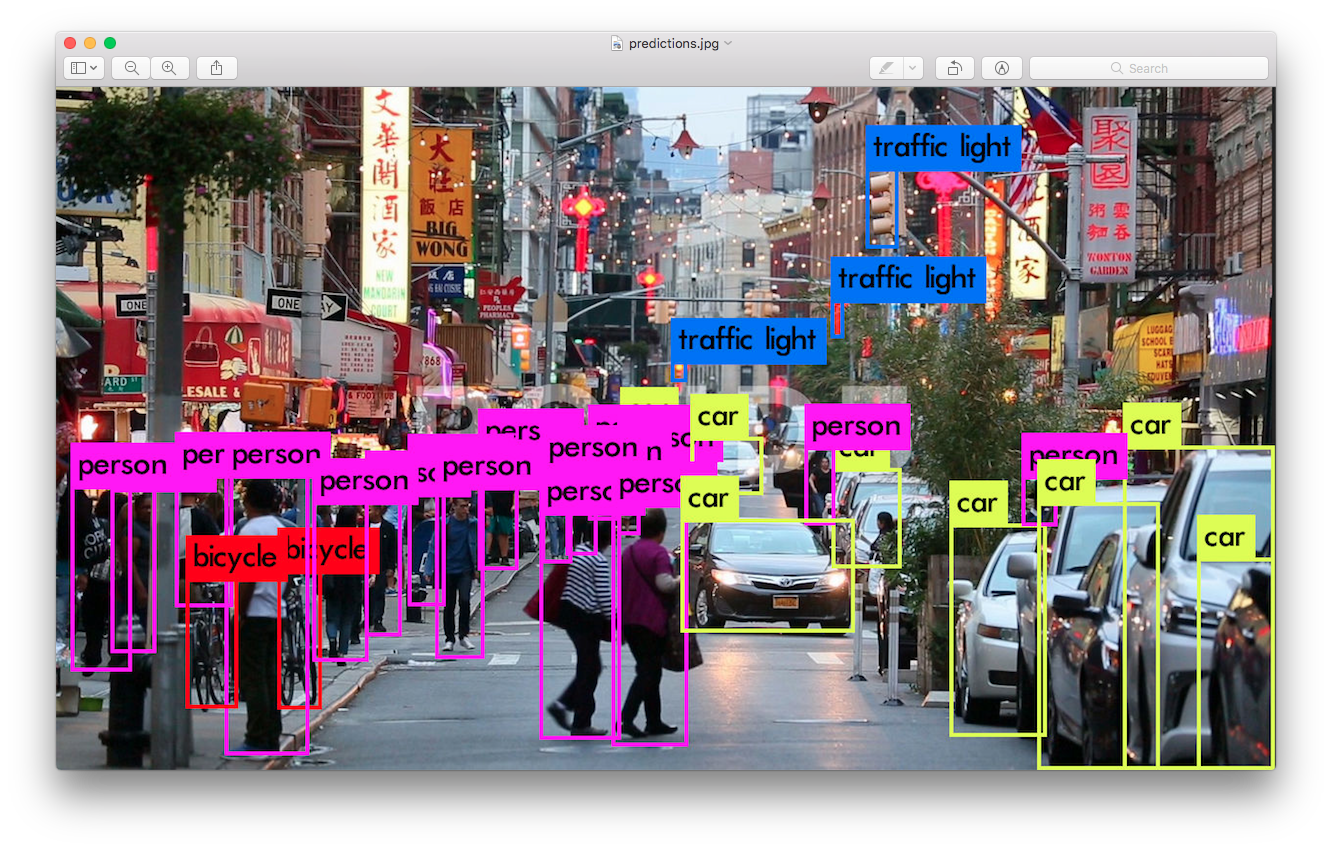
\includegraphics[scale=0.3]{Images/PredS1.png}}
    \caption{Basic overview of street, runtime: approx 29 seconds}
    \label{fig3}
\end{figure}

This first figure looks fine, and indeed, with basic weights, what we expect is outlined, although notable items like height changes, curbs, poles and whatnot are not outlined, everything else is decently well done. However, the runtime is still pretty staggering, so I tried the fast running YOLOv3-nano architecture. \textit{(Keep in mind v3 is from 2018 and is deprecated now as v4 was just released, but I already have these images and I'm just trying to make a point.)}

\begin{figure}[htbp]
    \centerline{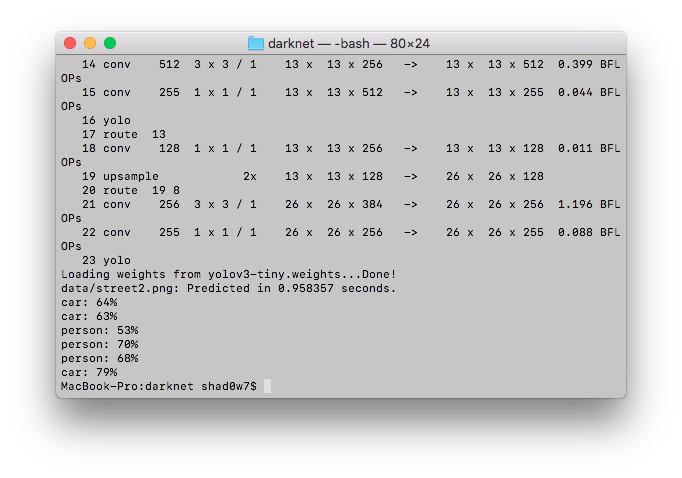
\includegraphics[scale=0.5]{Images/Term2.png}}
    \caption{Same test image, runtime 0.9s}
    \label{fig4}
\end{figure}

This is more promising, the runtime is still around 1FPS but this is like Intel from 2012, according to the people that make the software, GPU's are also much faster. The unfortunate truth is, that the output isn't promising like at all.

\begin{figure}[htbp]
    \centerline{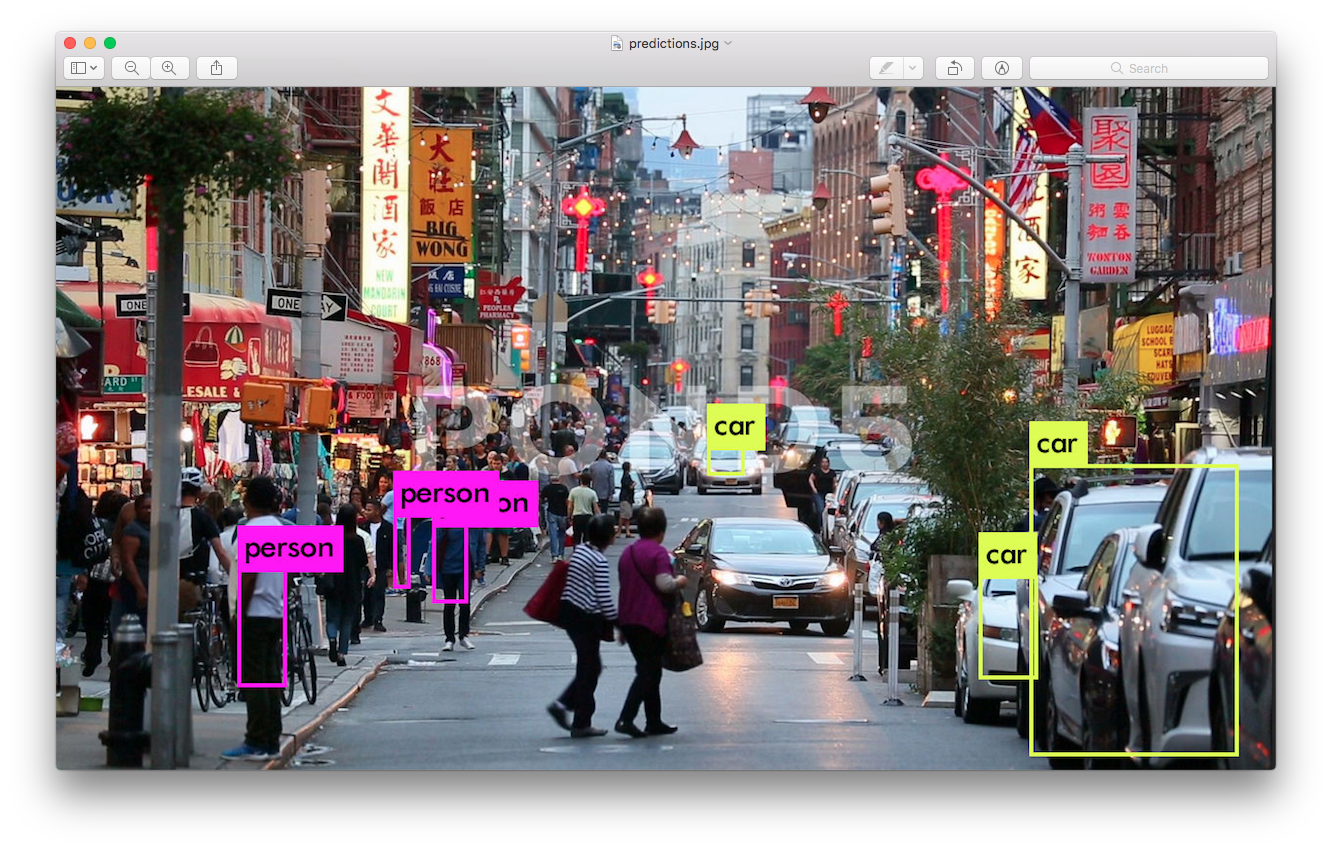
\includegraphics[scale=0.3]{Images/PredS4.png}}
    \caption{Not great detection.}
    \label{fig5}
\end{figure}

This is really not usable. However, back to 500x better, on a Jetson Nano, the GPU based workstation chip that I want to use, 15FPS is to be expected from the YOLOv3-nano, while 5FPS is with the full weights. Its only imperative that even less FPS would be gleaned from a trained model.

Hopefully Detecteron2 has better performance, and I will test this tomorrow on the same machine.

\textit{NOTE: My logic is that if it works better on an ancient (described as obsolete by Apple) no GPU hardware, it should work better on newer shinier hardware, so if Detecteron works faster on the same set of test images than YOLOv3, it should also work better on Jetson, as both use CUDA.}

\section{June 9th}

\end{document}